\documentclass{polytech/polytech}
\usepackage{amsmath}
% zone du préambule
\SetKw{Break}{break}


\typereport{custom}
\typereportname{Rapport de projet développement DII3}

\reportyear{2017-2018}
\schooldepartment{dii}

\title{Outil d'aide à l'affectation des projets}

\student[dii3]{Jérémy}{Loche}{jeremy.loche@etu.univ-tours.fr}
\student[dii3]{Louis}{Thomas}{louis.thomas@etu.univ-tours.fr}

\academicsupervisor[dii]{Ameur}{Soukhal}{ameur.soukhal@univ-tours.fr}

\motcle{affectation}
\motcle{solver}
\motcle{modèle}
\motcle{mathématique}
\motcle{google}
\motcle{sheet}
\resume{Ce projet a pour but de fournir un outil d'aide a l'affectation des projets.}

\keyword{example}
\keyword{\LaTeX}
\abstract{This is an example of an abstract for the report.}

\posterblock{Constat}{Plein de truc sont à améliorer dans ce projet}{images/modeemploi}{}
\posterblock{Solution}{Il y en a plein :
\begin{itemize}
    \item la première
    \item la deuxième
\end{itemize}
}{images/fig1}{}

\posterblock{Conclusion}{Tout marche nickel}{images/fig2}{Ma légende}

\addbibresource{biblio}



\begin{document}
% zone du contenu du document

%=========BEGIN chap 0=============
\chapter*{Introduction}
\label{chap:intro}

Tous les ans, dans toutes les promotions d'étudiants ingénieurs de Polytech Tours, d'intenses débats ont lieu au moment des affectations de projets. En effet, chacun souhaite avoir le projet qui lui plaît le plus. Pour aider à dénouer ces débats, nous avons proposé de travailler sur un outil d'aide à l'affectation des projets étudiants. 

A travers ce projet, nous verrons comment nous avons choisi de résoudre problème d'affectation afin que chacun soit satisfait de son affectation.

Vous découvrirez comment nous avons réparti notre charge de travail dans ce développement.

Nous aborderons alors comment nous avons modélisé ce problème puis avec quels outils nous avons travaillé pour arriver à un outils de saisie et de résolution des affectations.

Pendant la lecture de ce rapport de projet, nous vous exposerons une méthode de résolution du problème d'affectation.

%=========BEGIN chap 1=============
\chapter{Le problème d'affectation}
\label{chap:pb_affectation}

\section{Présentation}
\label{sec:pres_affectation}

Ce travail est un problème d'affectation.
En effet, le but est d'associer à un ou plusieurs individus un projet précis en respectant un objectif simple: maximiser la satisfaction générale de l'affectation.
L'idée et que chacun soit satisfait du projet auquel il a été affecté et qu'il soit en mesure de le mener à bien dans les meilleures conditions.


\section{La modélisation mathématique}
\label{sec:mod_math}

Pour résoudre ce problème, nous allons avoir besoin de la formaliser de manière mathématique afin d'essayer de trouver des solutions.
Nous rappelons que le but est d'affecter un étudiant, un binôme ou un groupe de personnes à un projet.

Le fait de formaliser un problème en langage mathématique nous permettra de demander à un \textbf{solver} de trouver la solution à notre problème.

Pour cela, il faut définir quels sont les \textbf{paramètres}\footnote{Dans un modèle mathématique, un paramètre est une donnée.}, les \textbf{ variables}\footnote{Dans un modèle mathématique, une variable est une valeur calculée, une inconnue.}, les \textbf{contraintes}\footnote{Les contraintes représentent les règles à respecter lors de la résolution du problème.}, et la \textbf{fonction objectif}\footnote{C'est l'ultime but à atteindre pour établir que la solution au problème est optimale.} de notre problème.

Commençons par définir nos données c'est à dire les paramètres de notre modèle.

\subsection{Les données et les paramètres}
\label{sec:donnees_params}
Pour cela on commence par créer deux entités appartenant à deux ensembles qui seront nos données de départ:
\begin{enumerate}
\item une entité $individu \in Individus$ : représente une personne, un binôme ou un groupe de personnes qui accomplira un \textbf{projet};
\item une entité  $projet \in Projets$ : représente un projet auquel sera affecté un \textbf{individu}.
\end{enumerate}

Pour plus de simplicité, on va indicer les entités comme dans \autoref{tab:indice_entite_mod_math}. On a choisi que les binômes seront représentés par des individus.
\begin{table}
\caption{\label{tab:indice_entite_mod_math}Indiçage des entités du modèle mathématique}
\begin{tabular}{|c|c|c|c|}
\hline
\multicolumn{2}{|c|}{$\forall individu \in Individus$} & \multicolumn{2}{|c|}{$\forall projet \in Projets$} \\
\hline
\textbf{Indice Individu} & Nom individu &\textbf{ Indice Projet} & Nom projet \\
\hline
\textbf{1} & Binôme: Arthur, Léo & \textbf{1} & Projet: Lampe connecté \\
\hline
\textbf{2} & Binôme: Sophie, Jean & \textbf{2} & Projet: Moniteur UVA \\
\hline
... & ... & ... & ... \\
\hline
\textbf{nbIndividus} & Binôme: Paul, Pierre &\textbf{ nbProjets} & Projet: Voiture RC \\
\hline
\end{tabular}
\end{table}

Pour que l'affectation de chaque individu à un projet, il faut assez de projet pour tout le monde ce qui implique la relation suivante:
$$ nbProjets \geqslant nbIndividus$$

Pour tout les individus, on souhaite connaître sa préférence pour un projet afin de procéder à l'affectation. En utilisant le formalisme mathématique, on peut définir la quantité $preference$ qui définira l'appréciation d'un individu à un projet donné:
$$
\forall (i,p) \in Individus \times Projets,
preference[i,p] \in \llbracket 1, nbProjets \rrbracket
$$
On choisit de dire que cette préférence va de $nbProjet$ à 1 dans l'ordre décroissant d'appréciation. Ainsi, un individu qui aurait la préférence $nbProjets$ pour un projet indiquera que ce projet est son préféré et 1 pour celui qui lui plait le moins.

Pour que l'affectation soit équitable, un individu ne peut pas donner la même préférence à deux projets différents. De manière mathématique cela donne:
$$
\forall (i,p1,p2) \in Individus \times Projets^2 , p1 \neq p2 \Rightarrow preference[i,p1] \neq preference[i,p2]
$$

Lorsque ces pré-conditions sont respectés, alors on crée un \textbf{paramètre} appelé préférence utile pour résoudre le problème d'affectation.
$$
\forall (i,p) \in Individus \times Projets,
preference[i,p]
$$

Nous allons maintenant voir quels contraintes et variables sont à déterminer pour résoudre le problème.

\subsection{Les variables et les contraintes}

Pour modéliser entièrement le problème d'affectation, la préférence de chaque individus pour un projet n'est pas suffisante.
%todo
Nous allons devoir mettre en place des \textbf{ variables} et des \textbf{contraintes} qu'elles doivent respecter.

Une \textbf{variable} est une valeur qui doit être déterminée pour résoudre le problème. Il faut donc la calculer.

Nous cherchons à déterminer a quel projet est affecté un individu. Pour cela on crée la variable $affectation$:
$$
\forall (i,p) \in Individu\times Projets , affectation[i,p]=
\left\lbrace
\begin{array}{l}
1 \text{ si l'individu i est affecté au projet p} \\
0 \text{ sinon}
\end{array}
\right.
$$

On connait la quantité que l'on souhaite déterminer pour résoudre le problème d'affectation, cependant, il faut définir des \textbf{contraintes} qui vont définir les règles de l'affectation.

Nous allons énoncer et définir deux contraintes utiles à la résolution du problème. La première est le nombre de projets par individus et la seconde est le nombre d'individus par projets.
Pour une affectation d'un individu pour un projet, alors on a les contraintes \eqref{eqn:nb_proj_indiv} et \eqref{eqn:nb_indiv_proj}.

\begin{equation}
\label{eqn:nb_proj_indiv}
\forall i \in Individus, nbProjetsParIndividu= \sum_{p \in Projets} affectation[i,p] = 1
\end{equation}

Pour notre problème, un individu doit être affecté à un seul projet, ce qui donne la contrainte \eqref{eqn:nb_proj_indiv}.

\begin{equation}
\label{eqn:nb_indiv_proj}
\forall p \in Projets, nbIndividusParProjet= \sum_{i \in Individus} affectation[i,p] \leqslant 1
\end{equation}

La contrainte \eqref{eqn:nb_indiv_proj} dit qu'un projet ne peut être réalisé que par au plus un individu.

Nous avons définit nos paramètres, variables et contraintes, donc il ne reste plus qu'à définir l'objectif à atteindre avec tout ça.
\subsection{Objectif simple, maximiser la préférence moyenne}
\label{sec:max_pref_moy}

Pour choisir quelle configuration de variable on va garder, c'est à dire quel choix d'affectation on va faire, on va devoir mettre en place un indicateur permettant de juger de la qualité de l'affectation.
On appelle cet indicateur la \textbf{fonction objectif}.
Trouver la solution à un problème mathématique se résume souvent à établir la bonne fonction objectif qu'on souhaite faire converger vers une valeur donner, maximiser ou minimiser.


Dans notre cas, on souhaite maximiser la satisfaction générale, c'est à dire maximiser la somme des préférence des projets affectés à chacun. Ainsi le résultat optimal sera atteint lorsqu'on aura réussi a trouver la combinaison de variable qui donne la plus grande valeur de la \textbf{fonction objectif}.

\begin{equation}
\label{eqn:maximize_preference}
\text{maximiser} \left( \sum_{(i \in Individus)} \sum_{(p\in Projets)} affectation[i,p]\times preference[i,p] \right)
\end{equation}

Pour le problème d'affectation maximiser la fonction objectif \eqref{eqn:maximize_preference} donnera la satisfaction générale la plus élevée car elle correspondra à faire en sorte que si un individu est affecté à un projet, la valeur de la préférence sera en moyenne la plus grande.

Cette méthode fonctionne est efficace pour trouver la meilleur préférence moyenne, cependant, elle peut être injuste et sélectionner pour la majorité des individu la préférence maximale et pour un individu la pire des préférence.

Il peut donc apparaître un sentiment d'injustice derrière cette affectation avec la sensation que quelqu'un à été mis de coté pour satisfaire le bien commun.

A cela, nous proposons un solution de compromis qui fourni une solution plus homogène (si elle existe évidemment).

\subsection{Objectif de compromis, la contrainte de la préférence minimale}
\label{sec:pref_min}

Pour obtenir une affectation plus homogène, on introduit une contrainte au modèle: c'est la contrainte de la préférence minimale.
Le but est d'assurer que lorsqu'un individu est affecté à un projet, la préférence soit supérieure ou égale à une valeur de seuil $ValeurPrefMin$.
On peut donc assurer avec cette contrainte que la préférence n'atteindra jamais 1 ou 2 etc...

On pose donc un nouveau \textbf{paramètre}:
$$
ValeurPrefMin \in \llbracket 1,nbProjet \rrbracket
$$

Et une nouvelle \textbf{contrainte}, qui impose que l'affectation soit faite avec un préférence supérieure à $ValeurPrefMin$ :
$$
\forall i \in Individus ,preferenceMinimale = \sum_{p \in Projets} affectation[i,p]\times preference[i,p] \geqslant ValeurPrefMin
$$

\paragraph{Problème} Cette contrainte est très restrictive sur les solutions. Il se peut même $ValeurPrefMin$ de manière trop audacieuse et que le problème soit insoluble avec ces paramètres.
Prenons un exemple de l'affectation de 4 individus et 4 projets (Cf. \autoref{tab:preference_exemple}).

\begin{table}
\caption{\label{tab:preference_exemple}Données de préférence pour l'exemple}
\begin{tabular}{|c|c|c|c|c|}
\hline
préférence[individu,projet] & Projet 1 & Projet 2 & Projet 3 & Projet 4 \\
\hline
Individu 1 & 4 & 3 & 2 & 1 \\
\hline
Individu 2 & 4 & 3 & 1 & 2 \\
\hline
Individu 3 & 3 & 4 & 2 & 1 \\
\hline
Individu 4 & 2 & 4 & 1 & 3 \\
\hline
\end{tabular}
\end{table}

Si on choisi $ValeurPrefMin=3$, alors le modèle mathématique est insoluble car la contrainte $preferenceMinimale$ ne pourras pas être respectée pour tout les individus. On a 4 projets pour 4 individus, on remarque qu'il faudra donc exactement 1 projet par individu pour respecter la contrainte $nbProjetsParIndividu=1$. Le problème est que si un individu est affecté au projet P3, alors la valeur de la préférence est inférieure ou égale à 2 donc inférieure à $ValeurPrefMin=3$. On ne respecte alors pas la contrainte $preferenceMinimale$ pour un des individu donc le modèle est insoluble.
Pour trouver une solution il faudra revoir le paramètre $ValeurPrefMin$ à la baisse. Pour la valeur 2, on commencera a trouver des solutions pour laquelle la $ValeurPrefMin$ est maximale. Donc les bonnes solutions de compromis.

Il y a plusieurs solutions pour automatiser la détermination de la valeur de $ValeurPrefMin$ pour laquelle on assure que tout le monde aura la meilleur préférence possible tout en maximisant la satisfaction générale.

\paragraph{Solution 1}
Le but est d'essayer de trouver la valeur maximale de $ValeurPrefMin$ pour laquelle on arrive a résoudre le modèle. Pour cela, on peut rechercher la valeur maximale en faisant plusieurs résolutions du modèle mathématique en fixant différentes valeurs de $ValeurPrefMin$. On peut faire une recherche par tentative ou dichotomique. $ValeurPrefMin$ n'intervient pas dans la fonction objectif à ce stade.

\subparagraph{Recherche de $ValeurPrefMin$ par tentative}

La fonction $SolveModel(\text{param:} ValeurPrefMin)$ est un sous-algorithme appelé par notre algorithme pour effectuer la résolution du modèle mathématique avec la valeur de préférence minimale passée en paramètre.
Elle renvoie une structure $ResultSolver$ contenant les résultats de la résolution $ResultSolver.data$ et l'état de la résolution $ResultSolver.state$ qui peut valoir soit $Success$ si une solution au modèle a été trouvée et $Fail$ sinon.

On l'utilise donc pour savoir si on a réussi a résoudre le
\begin{algorithm}
\caption{\label{chap:problem_affectation:algo:recherche_tatonnement}Résolution du modèle avec $ValeurPrefMin$ choisi par tentative}

\tcc{Init variable résultat du solver, contient $ResultSolver.data$ et $ResultSolver.state$}
$ResultSolver \gets Null$ \\

\tcc{Commencer par la valeur la plus restrictive jusqu'à la moins restrictive}
\For{$ValeurPrefMin=nbProjets$ \KwTo $1$}
{

	\tcc{Effectuer une résolution avec la valeur de préférence minimale}
	$ResultSolver \gets SolveModel(ValeurPrefMin)$ \\



	\If{$ResultSolver.state= Success$}
	{
		\tcc{Le solver a trouvé une solution}
		\tcc{on a trouvé le maximum pour $ValeurPrefMin$}
		\tcc{on arrête la boucle ici}
		\Break

	}
}
\tcc{Retourner le résultat du solver qui est donc la solution avec la $ValeurPrefMin$ maximale et la plus grande satisfaction}
\Return{ResultSolver}
\end{algorithm}

Cette méthode n'a pas la meilleur complexité et peut considérablement allonger les temps de résolution du modèle. C'est pour cela que nous proposons la méthode dichotomique.

\subparagraph{Recherche de $ValeurPrefMin$ dichotomique}
\begin{algorithm}
\tcc{Init variable résultat du solver, contient $ResultSolver.data$ et $ResultSolver.state$}
$ResultSolverFinal \gets Null$ \\
$deb \gets 1$ \\
$fin \gets nbProjet$ \\
$mil \gets \frac{deb+fin}{2}$ \\
\While{$deb<fin$}
{
	$ResultSolverTemp=SolverModel(mil)$\\
\If{$ResultSolverTemp.state=Success$}
{
$deb=mil+1$\\
$ResultSolverFinal=ResultSolverTemp$\\
$mil \gets \frac{deb+fin}{2}$ \\
}
\Else
{
	$fin=mil-1$\\
	$mil \gets \frac{deb+fin}{2}$ \\
}
}

\Return{$ResultSolverFinal$}
\caption{\label{chap:problem_affectation:algo:recherche_dichotomique}Recherche de $ValeurPrefMin$ dichotomique}
\end{algorithm}
\paragraph{Solution 2}
On change la nature de $ValeurPrefMin$ et elle devient donc une \textbf{variable} intervenant dans la fonction objectif.
L'idée derrière cette modification est de demander, en plus de la maximisation de la préférence moyenne, une maximisation de la $ValeurPrefMin$.

\subparagraph{Méthode par aggrégation}
On peut rajouter $ValeurPrefMin$ dans la fonction objectif en faisant une simple somme (Cf. \eqref{eqn:max_obj_aggregation})

\begin{equation}
\label{eqn:max_obj_aggregation}
\text{maximiser} \left( ValeurPrefMin + \sum_{(i \in Individus)} \sum_{(p\in Projets)} affectation[i,p]\times preference[i,p] \right)
\end{equation}

Cette agrégation permettra donc de chercher aussi a maximiser la $ValeurPrefMin$. Cependant, elle ne le sera pas au même titre que la satisfaction moyenne car il peut être plus avantageux de chercher à maximiser d'avantage la satisfaction que la $ValeurPrefMin$.

\subparagraph{Méthode de combinaison linéaire des variables}
Pour cela, on peut ajouter des poids $\alpha, \beta$ deux nombres donnés qui peuvent servir à donner plus d'importance à la $ValeurPrefMin$ ou à la satisfaction générale (Cf. \eqref{eqn:max_obj_combi_lineaire}).

\begin{equation}
\label{eqn:max_obj_combi_lineaire}
\text{maximiser} \left( \alpha ValeurPrefMin + \beta \sum_{(i \in Individus)} \sum_{(p\in Projets)} affectation[i,p]\times preference[i,p] \right)
\end{equation}


\paragraph{Transition:}
Après avoir vu le fond du problème que nous avons souhaité résoudre dans ce projet, nous allons passer à notre proposition de réalisation d'un outil d'aide à l'affectation des projets.
%=========END chap 1================


%=========BEGIN chap 2================
\chapter{Organisation et choix techniques de réalisation de l'outils d'affectation}



\section{Résoudre le problème d'affectation}
Il existe plusieurs manières de résoudre le problème d'affectation.
Nous rappelons que le but est d'attribuer pour chaque étudiant un unique projet en maximisant la satisfaction générale.

Dans un premier temps, nous avons recherché des algorithmes permettant de résoudre ce problème. Nous verrons 2 méthodes, l'une utilisant un algorithme Hongrois et l'autre utilisant un solver linéaire.

\subsection{L'algorithme Hongrois, de Kuhn-Munkres}

L'algorithme Hongrois permet de trouver un couplage parfait dans un graphe biparti de poids maximum (ou minimum) d'après Wikipédia.

\paragraph{Pourquoi est-ce un algorithme adapté au problème d'affectation ?}

\subparagraph{Un graphe biparti ? Pourquoi ?}
Un graphe biparti un type particulier de graphe dont on distingue 2 nuages de noeuds dont les noeuds appartenant à un nuage ne peuvent être lié qu'aux noeuds de l'autre nuage par des arcs. 
Autrement dit, il est interdit d'avoir un arc entre 2 noeuds d'un même nuage.

\begin{figure}[htbp]
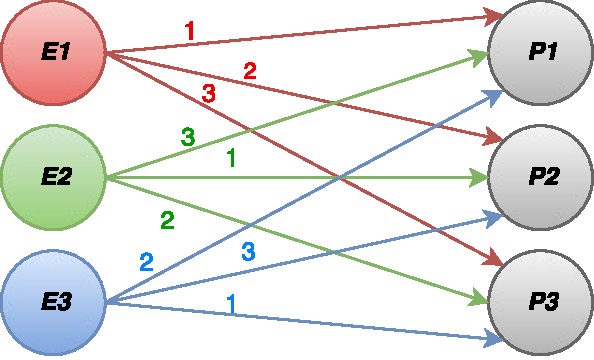
\includegraphics[width=8cm]{images/Graphe_bipartie}
\caption{\label{fig:graphe_biparti}Modélisation étudiants-projets dans un graphe biparti complet}
\end{figure}

On a une analogie directe entre les 2 nuages de noeuds du graphe, le premier nuage représente les étudiants et le second représente les projets.

Chaque étudiant est lié à chaque projets par $n$ arcs pour les $n$ projets. Par exemple dans la \autoref{fig:graphe_biparti}, on dispose de 3 étudiants ayant émis une préférence pour chaque projets. La valeur de la préférence correspond au poid sur l'arc reliant l'étudiant au projet.

\subparagraph{Un couplage parfait ? \`A quoi ça correspond ?}

Un couplage parfait dans un graphe correspond à choisir des arcs dans ce graphe de façon à ce qu'il n'existe qu'un et un seul arc entre chaque noeuds.
Dans notre cas, si on réalise un couplage parfait sur le graphe biparti, alors on aura réalisé une affectation des étudiants à un projet. 

\begin{figure}[htbp]
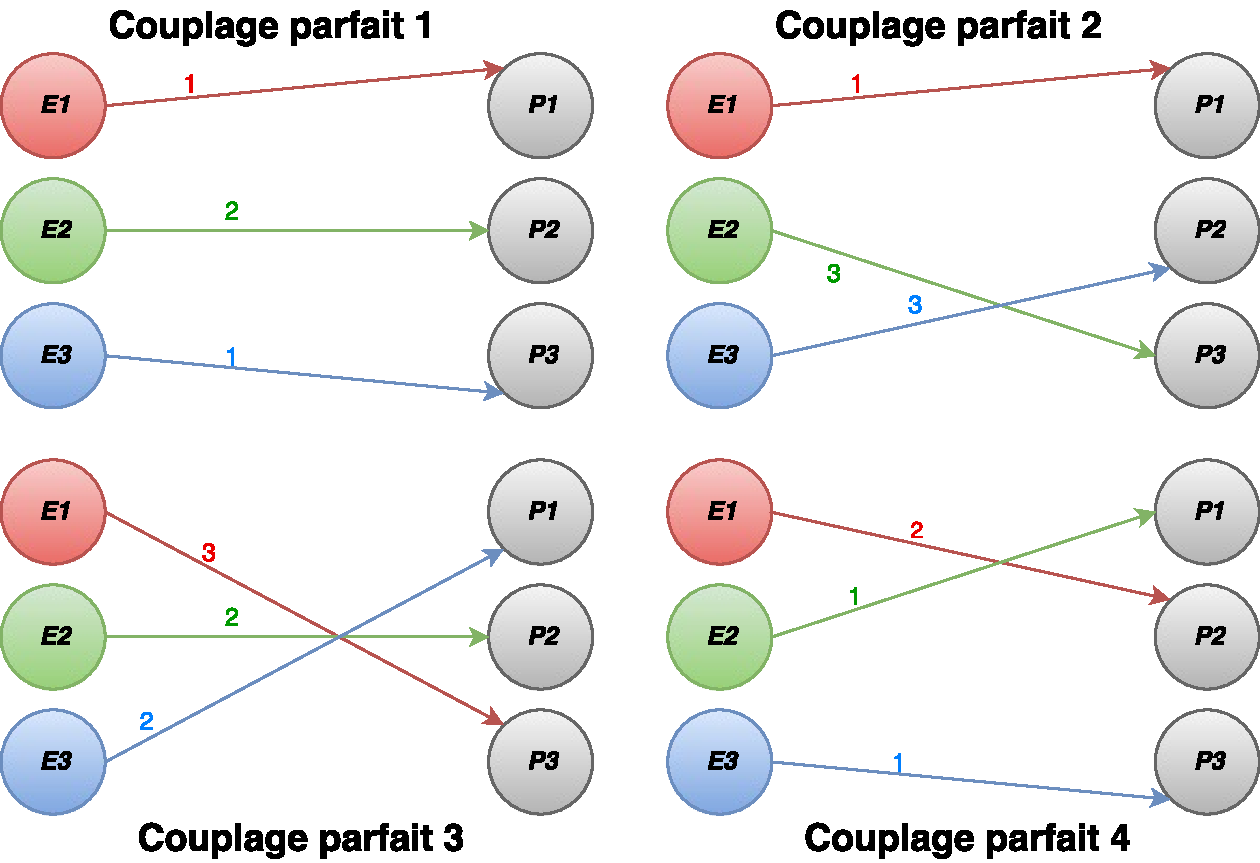
\includegraphics[width=12cm]{images/graphe_biparti_couplage_parfait}
\caption{\label{fig:graphe_biparti_couplage_parfait}Couplages parfait sur le graphe biparti (\autoref{fig:graphe_biparti})}
\end{figure}

La \autoref{fig:graphe_biparti_couplage_parfait} illustre ces propos en mettant en évidence quelques couplages possibles à partir du graphe biparti (\autoref{fig:graphe_biparti}).

La méthode hongroise de résolution permet alors de trouver le couplage parfait maximisant (ou minimisant) la somme des poids de tous les arcs du couplage.

Pour nous, cela correspond à trouver les affectations qui satisfont tout le monde ! 

Nous ne rentrerons pas dans les détails de l'implémentation de l'algorithme hongrois car ce n'est pas la solution que nous avons retenu pour effectuer nos calculs d'affectation. 

Nous l'avons toutefois testé lors du démarrage du projet en déroulant l'algorithme à la main sur un petit jeu de données et en utilisant une \textit{librairie Munkres} implémentant la méthode hongroise sur \textit{python} et \textit{JavaScript}.

De la littérature très bien écrite est disponible sur Internet avec notamment: TODO AJOUTER LES REFERENCES
%TODO

Nous nous sommes rapidement tourné vers l'optimisation par programmation linéaire plus flexible en termes de contraintes pour la résolution des problèmes et pour laquelle il existe de très puissants algorithmes implémentés dans des logiciels optimisés.

En effet, si résoudre le problème d'affectation comme le fait la méthode hongroise revient à résoudre le problème linéaire que nous avons définit au \autoref{chap:pb_affectation}.

La seule différence est que seules les contraintes \autoref{eqn:nb_indiv_proj} et \autoref{eqn:nb_proj_indiv} sur le nombre de projets par étudiants et le nombre d'étudiants par projet est fixé à $1$ pour que la méthode hongroise soit applicable.
De même la fonction objectif de ce problème sera forcément \autoref{eqn:maximize_preference}. La compléxité de cet algorithme est comprise entre \textbf{O($n^3$)} et  \textbf{O($n^4$)}, c'est à dire qu'elle s'exécute en un temps proportionnel au polynôme $n^3$ ou $n^4$ avec $n$ la dimension de la matrice \textit{affectation} à déterminer.

Le besoin de changer de méthode résolution et la nécessité de passer à la programmation linéaire est apparu lorsque nous avons commencé a ajouter des contraintes à notre modèle.

Nous allons voir désormais comment l'optimisation linéaire permet de résoudre le problème.

\subsection{Résolution par un Solver Linéaire}
%TODO parler du solver glpk et les méthodes de résolutions.

Pour résoudre le problème d'affectation, après avoir testé la méthode Hongroise, nous avons découvert le solver GLPK qui permet de résoudre les problèmes d'optimisation linéaire.

Un \textbf{solver linéaire}  est un machine à calculer équipé d'algorithmes d'optimisation permettant de trouver la solution à un modèle mathématique qui maximise (minimise, ou se rapproche d'une valeur donné) au mieux la fonction objectif qui est combinaison linéaire des variables à déterminer.

Tel que nous l'avons défini, le problème d'affectation est \textbf{un problème d'optimisation linéaire}. 

Ce qui peut rendre la résolution du problème compliqué est le fait que les \textbf{variables de décision}, dans notre cas les \textit{affectations} doivent être des nombres entiers. En effet, un étudiant ne peux pas être affecté à 0,5 projet.

Comme il s'agit d'un problème dont les solutions sont des nombres entiers, nous avons utilisé la programmation linéaire en nombre entiers (PLNE) pour le résoudre. 

Un problème de programmation linéaire en nombre entiers est construit de la même façon que dans le \autoref{chap:pb_affectation}. 

Il faut fournit un jeu de \textbf{paramètres} au problème, \textbf{variables} de décisions, \textbf{contraintes} et enfin une \textbf{fonction objectif}.

%TODO (Par soucis de légèreté du rapport nous n'exposerons pas toutes les méthodes permettant de trouver quelle solution maximise au mieux la fonction objectif.)

Une façon naïve de résoudre le problème serait de procéder par itération en listant toutes les valeurs possibles des variables à déterminer et de les tester une par une. 

Alors il suffira de voir si une valeur donnée respecte toutes les contraintes et obtient une meilleur note à la fonction objectif.

 Si c'est le cas, alors on gardera cette solution jusqu'à en trouver une meilleure où lorsque l'on aura testé toutes les possibilités.

Il y a un gros problème de performances avec cette méthode, car pour notre problème, la matrice des \textit{affectations} a une taille de $nbProjets\times nbIndividus$ et ne contient que des 0 et des 1.

Un calcul rapide nous permet de dire qu'il existe $2^{nbProjets\times nbIndividus}$ combinaisons de la matrice \textit{affectations}.
En prend $nbProjets=nbIndividus=n$, c'est à dire autant d'élèves que de projets.

La complexité de cette recherche de la meilleure solution est de \textbf{O($2^{(n^2)}$)}, ce qui est vraiment mauvais même pour de très petit échantillons. Le temps de résolution sera exponentiel en fonction de la taille des données d'entrée.

\begin{equation}
n=4
\left(
\begin{array}{cccc}
1 & 1 & 1 & 0 \\ 
0 & 1 & 0 & 1 \\ 
0 & 1 & 1 & 1 \\ 
1 & 1 & 1 & 0
\end{array} 
\right)
\text{Exemple de matrice pour affectation}
\end{equation}

Parmi les valeurs possible de la matrice d'affectations, nombreuses sont celles qui ne respecteront pas la contraintes d'un projet par étudiants ni même la contraintes d'un projet par étudiants. 

C'est a dire qu'il n'existe qu'au mieux 1 seul 1 sur chaque ligne et chaque colonne de la matrice.

On pourrait donc se servir de ces informations pour discriminer certaines des valeurs de la matrice \textit{affectations}.

Pour une matrice de taille $n\times n$, on ne peut construire qu'un dictionnaire de $n!$ matrices potentiellement solution du problème d'affectation. 

\begin{equation}
\left.
n=4
\begin{array}{cc}
\left(
\begin{array}{cccc}
1 & 0 & 0 & 0 \\ 
0 & 0 & 0 & 1 \\ 
0 & 1 & 0 & 0 \\ 
0 & 0 & 1 & 0
\end{array} 
\right)
&
\begin{array}{l}
\leftarrow 4=n \text{  positions dispo.}\\ 
\leftarrow 3=n-1 \text{  positions dispo.} \\ 
\leftarrow 2=n-2 \text{  positions dispo.}\\ 
\leftarrow 1=n-3 \text{  positions dispo.}
\end{array} 
\end{array}
\right\rbrace
n! \text{ matrices possibles}
\end{equation}

On peut désormais baser notre recherche itérative sur ces $n!$ matrices de la variable \textit{affectation}. La complexité de la recherche est désormais de  \textbf{O($n!$)}. Par exemple pour une matrice $4\times 4$ , une recherche itérative simple en testant toutes les combinaison amènerai à rechercher parmi $2^{4\times 4} = 2^{16}=65535$ matrices alors qu'après la discrimination des matrices ne pouvant pas être solutions, on a plus que $4!=24$ matrices à tester. 

Cette méthode est moins efficace que l'algorithme Hongrois qui s'exécute en \textbf{O($n^4$)} au pire.

Cependant cette première optimisation de la recherche de la meilleure affectation fait parti d'un des nombreux mécanismes d'optimisation utilisés par le solver.

Cet exemple était là pour illustrer la façon avec laquelle on peut rechercher la solution au problème en fonction d'un modèle donné.

Cependant, un solver est complexe et nous n'avons pas passé en revue toutes les méthodes d'optimisation pour notre problème.

Par la suite, nous vous présenterons le solver utilisé qui est GLPK, un solver linéaire avec des méthodes de résolution efficaces même pour de larges volumes de données.

\section{Implémentation de la méthode de résolution}
%TODO Expliquer comment on a programmé le GLPK ? Fichier .dat et .mod, contenu du fichier mod et fichier dat

Pour mettre en application notre modèle mathématique, nous avons choisi d'utiliser le solver linéaire \textbf{GLPK} et d'écrire notre modèle en \textbf{GMPL} aussi connu sous le nom de \textbf{Mathprog}.

En effet, nous avons précédemment formalisé le modèle du problème d'affectation et il ne reste plus qu'à le traduire en langage informatique pour qu'un solver trouve une solution optimisée qui respecte toutes les contraintes.

Nous avons choisi GLPK car c'est un solver linéaire libre multi-plateforme qu'il est possible d'intégrer dans tout type d'applications à travers des librairies. L'avantage premier étant est qu'il est adapté à la résolution de notre problème linéaire.

Lors de ce projet, nous n'avons pas fait le tour de toutes les méthodes d'optimisations utilisées par les solver, nous avons surtout cherché à comprendre comment utiliser le solver et le langage GMPL pour l'utiliser à la résolution de notre problème.
 
Le langage GMPL est un langage de programmation linéaire haut niveau permettant de mettre en forme un modèle mathématique très facilement pour qu'il soit résolu par le solver GLPK.

Ce langage a été pensé pour être très proche du formalisme mathématique.

Il est possible avec GLPK de séparer données et modèle mathématique. 

En effet, on peut disposer d'un fichier \textbf{[Mon\_Modèle].mod} et lui associer des données \textbf{[Mes\_Données].dat}.

On peut ensuite appeler GLPK simplement via la commande:
\begin{center}
\textbf{glpsol -m \textit{[Mon\_Modèle]}.mod -d \textit{[Mes\_Données1]}.dat -d \textit{[Mes\_Données2]}.dat}
\end{center}

Vous trouverez en annexe  l'implémentation du modèle mathématique. TODO:RAJOUTER LE LIEN DU CODE GMPL assign.mod
%TODO

GLPK est disponible en librairie portable à cette adresse TODO AJOUTER LE LIEN GLPK online
%TODO

\section{Interface de saisie des données et création d'un back-end}
Dans cette partie du rapport, nous allons voir notre proposition en terme d'interface de saisie des préférences accompagnant notre modèle de résolution.

\subsection{Les choix et les objectifs}
Nous avons fait une étude sur les différentes possibilité de saisie (Excel, Google sheets, Celene, interface JAVA, console...).
Après avoir pesé les pour et les contres, nous nous sommes tourné vers \textbf{Google sheets} : une application web (un tableur similaire au logiciel excel Microsoft) faisant partie de la suite de google.
Une solution modulable permettant la saisie des voeux et des paramètres grâce à :
\begin{enumerate}
\item une mise en forme \textbf{flexible} et \textbf{évolutive}: l'outil tableur est très puissant;
\item une saisie \textbf{efficace} et \textbf{collaborative}: plusieurs étudiants peuvent modifier le tableur en même temps;
\item une mise en forme \textbf{intuitive} : affichage de notification et formulaire;
\item une accessibilité \textbf{simple} : un produit accessible gratuitement, via un lien et modifiable directement sans avoir besoin d'être connecté. Aucune installation n’est requise;
\item un langage de programmation \textbf{intuitif} : javascript;
\item un \textbf{support actif} avec documentation \textbf{soignée};
\item une total \textbf{liberté de communication} : appel d’api, lecture de fichiers, communication direct avec des pages html, création de modules.
\end{enumerate}

À propos de la résolution, nous avons fait le choix d’utiliser la librairie \textbf{GLPK} disponible dans plusieurs langage de programmation dont javascript. 

Avec des compétences en javascript et en connaissant le domaine des APIs, nous avons fait le choix de faire communiquer Google Sheets (l’interface de saisie) avec un serveur NodeJS qui comporte le framework \textbf{Express} utilisé en temps qu’API (Interface de Programmation Applicative\footnote{Une API est un logiciel utilisé pour résoudre un problème donné où répondre à un service permettant aux dévéloppeurs de ne pas se soucier de son implémentation.}).
 Ceci nous a mené à une  infrastructure d’application simple, moderne et puissante chargée de traiter les données envoyées par Google sheets.
L’avantage principal de l’API est le fait qu’elle peut être réutilisée pour d’autres projets. 
Par exemple, si une application mobile est créé pour résoudre le problème d’affectation, celle-ci pourra communiquer avec l’API.
En lui envoyant le bon format de donnée, celle-ci lui répondra avec les affectations. 

En effet, Google Sheets a une interface de développement appelé “Google Script” permettant d’effectuer des algorithmes en javascript.
C'est avec ce service que nous faisons appel à notre API.

La contrainte est que Google sheets ne communique pas avec des API local. Nous avons donc procéder à l'hébergement de cette application sur un domaine réservé : “testing-app.ovh/assign” et un serveur vps (serveur privé virtuel\footnote{Un VPS est une des nombreuses machine virtuelle hébergé sur une machine hôte puissante permettant d'avoir plusieurs serveurs sur une machine physique.}).

Cette api génère les données du modèle mathématique et les lie au \textbf{langage GMPL} (MathProg) en utilise une librairies intégrée GLPK pour le résoudre. 
La réponse est renvoyée en JSON à Google Sheets qui lui, se charge de l’afficher.

On peut résumer le fonctionnement global de notre logiciel à travers \autoref{fig:architecture_appli}.

\begin{figure}[htbp]
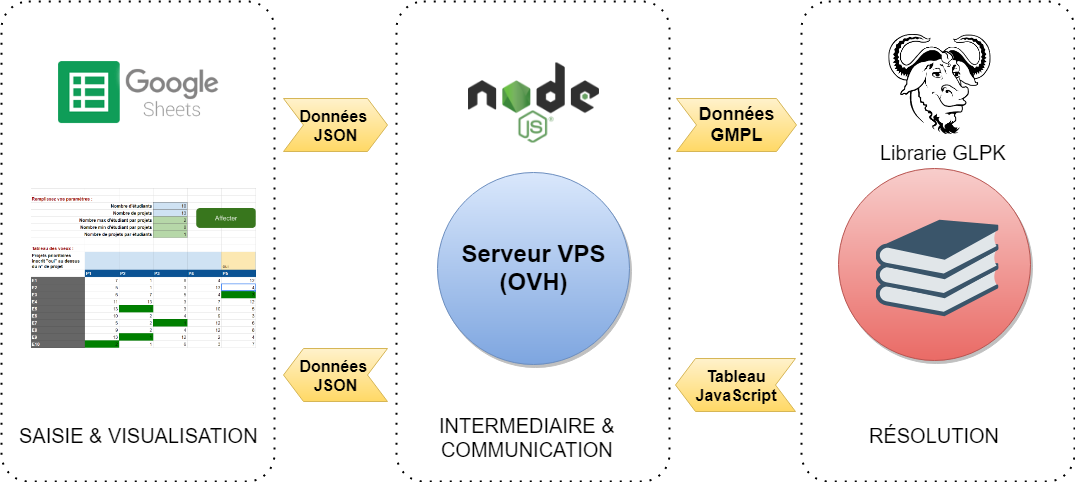
\includegraphics[width=15cm]{images/architecture_appli}
\caption{\label{fig:architecture_appli} Architecture de l'application de résolution des affectations}
\end{figure}

Sans plus attendre, nous allons entrer dans le vif du sujet et vous présenter l'interface que nous proposons.

\subsection{Réalisation de l'interface de saisie}

\begin{figure}
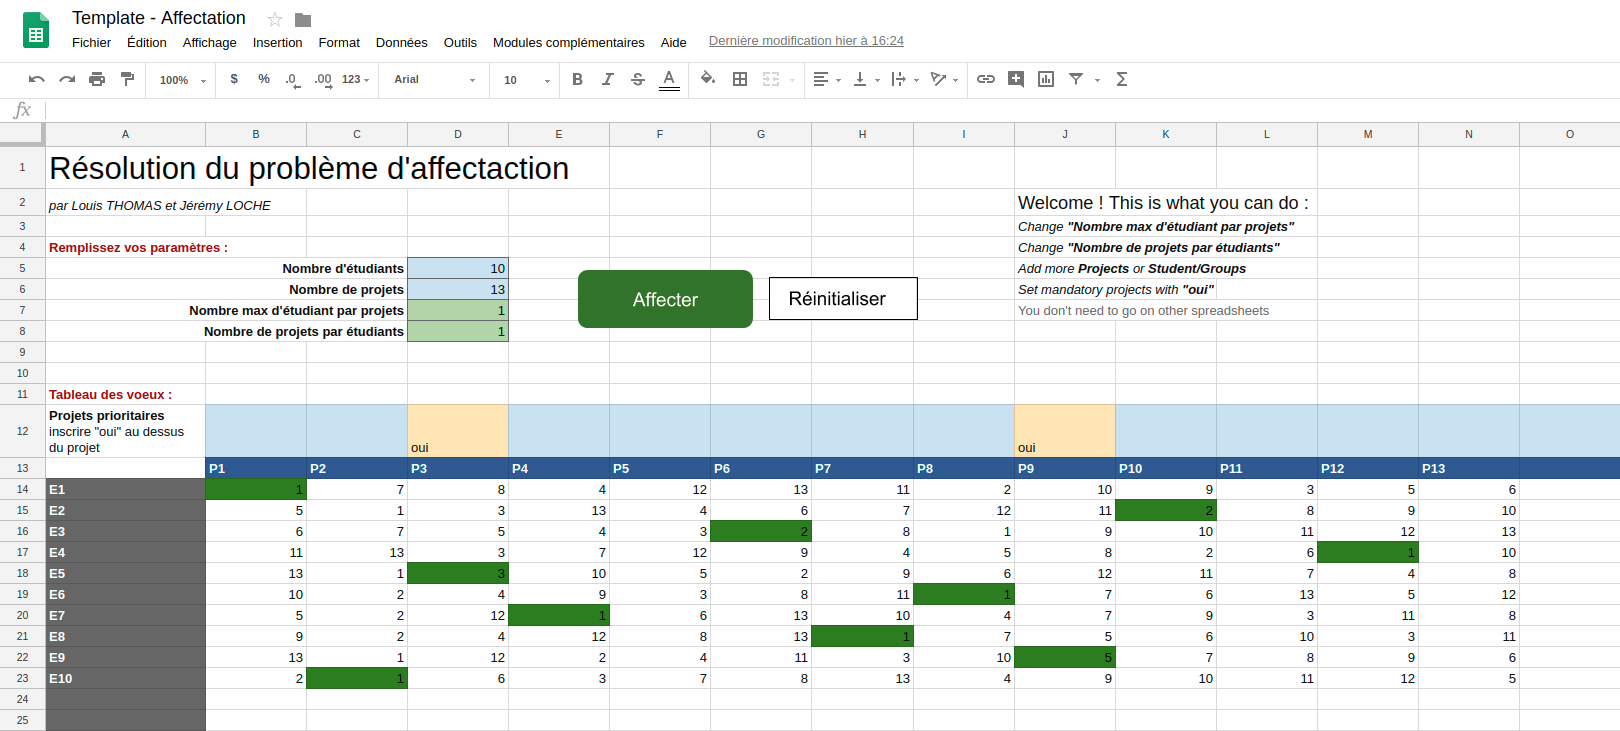
\includegraphics[width=15cm]{images/interface_appli_globale}
\caption{\label{fig:appli_interface_globale} Interface globale de l'application}
\end{figure}

La \autoref{fig:appli_interface_globale} présente l'interface de l'application dans sa globalité.
Elle dispose d'un tableau permettant à chaque élève/binôme ou groupe de pouvoir donner leurs voeux en fonction des projets (Cf. \autoref{fig:interface_preference}). Les voeux vont de 1 (le plus fort) jusqu’au nombre de projets.

\begin{figure}
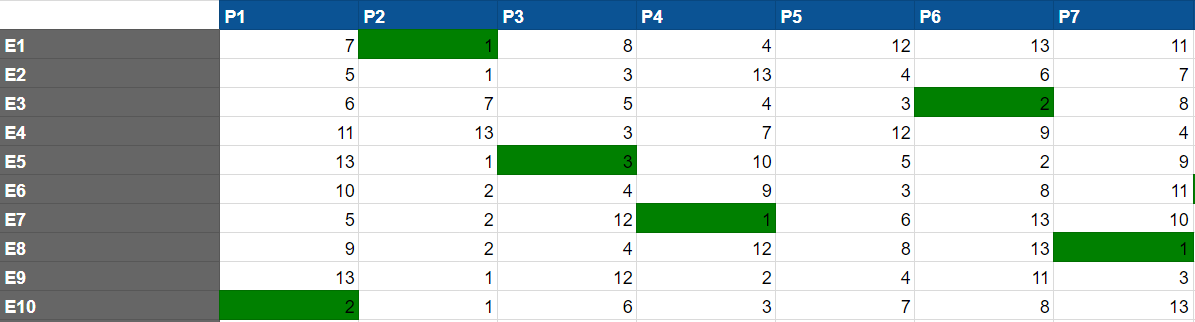
\includegraphics[width=15cm]{images/interface_preferences}
\caption{\label{fig:interface_preference}Tableau de saisie des préférences}
\end{figure}

Nous avons cherché a produire une interface simple et minimaliste.

L’utilisateur pourra également configurer les paramètres d'affectation affichés en vert (Cf. \autoref{fig:interface_parametres}):
\begin{enumerate}
\item Nombre max d’étudiant par projets
\item Nombre de projets par étudiants
\end{enumerate}

\begin{figure}
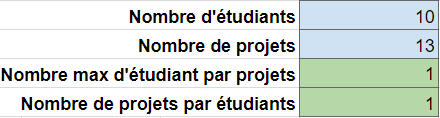
\includegraphics[width=12cm]{images/interface_parametres}
\caption{\label{fig:interface_parametres} Saisies des paramètres d'affectation}
\end{figure}



\subsection{Les améliorations}


%\section{Saisie et visualisation}
%TODO Comment programme google sheet, les outils utilisés pour tester, POSTMAN, node, serveur ovh...
%\section{Organisation Front et Back end}
%TODO Diagramme SYSML pour l'organisation du projet
%TODO Images des outils utilisés, GLPK, Google Sheets ,Node, Javascript, parsers java, python et Javascript...

%=========END chap 2================

\end{document}
